\documentclass[fleqn]{homework}

\student{Stephen Brennan (smb196)}
\course{EECS 440}
\assignment{Written 10}
\duedate{November 17, 2015}

\usepackage{enumerate}
%\usepackage{mathtools}
%\usepackage{graphicx}

\begin{document}
  \maketitle

  \begin{problem}{1}
    \begin{question}
      The Bayesian Candy Factory makes a Halloween Candy Box that contains a mix
      of yummy (Y) and crummy (C) candy. You know that each Box is one of three
      types: 1. 75\% Y and 25\% C, 2.  50\% Y and 50\% C and 3. 25\% Y and 75\%
      C. You open a Box and start munching candies. Let the
      $i\textsuperscript{th}$ candy you munch be denoted by $c_i$. Answer the
      following questions using MATLAB, R or any other math package. Generate
      one Box with 100 candies for each type, and assume a fixed order of
      munching. (1) For each Box, plot $Pr(T=i|c_1,\dots,c_N)$ on a graph where
      $T$ represents a type and $N$ ranges from 1 to 100. (You should have three
      graphs and each graph will have three curves.) (2) For each Box, plot
      $Pr(c_{N+1}=C|c_1,\dots,c_N)$ where $N$ ranges from 1 to 99. (3) Suppose
      you are an optimist, and before opening a Box you believe that each Box
      has 75\% Y (type 1) with probability 0.8 and the probability of the other
      two types is 0.1 each. Redo part (1) taking this belief into
      account. Briefly explain the implications of your results. (15 points)
    \end{question}

    For this situation, I have defined the probability of a list of candies
    $c_1, \dots, c_N$ given a box type as binomial, defining success as a Yummy
    candy, and failure as a Crummy one.  So, for example,
    $Pr[c_1, \dots, c_N|T=1]$ is binomial with parameters $N$ and $0.75$.  This
    is a slight simplification, since it models drawing candies with replacement
    from a population having the given statistics.  In reality, what is
    happening is that the box is drawn from such a population, and then candies
    are drawn with replacement from that box.  However, I believe that this
    simplification is reasonable for the purposes of this question's
    demonstration.

    Given this assumption, to compute the probability of a particular box type
    given candies, we simply apply Bayes' Rule:

    \begin{equation}
      Pr[T=i | c_1, \dots, c_N] = \frac{Pr[c_1, \dots, c_N | T=i] Pr[T=i]}{\sum_{i=1}^3 Pr[c_1, \dots, c_N|T=i] Pr[T=i]}
    \end{equation}

    These conditional probabilities are computed using the binomial distribution
    above.  We assume that $Pr[T=i]=\frac{1}{3}$ in parts 1 and 2, and then
    update this assumption in part 3.

    To compute the probability of the next candy being crummy given the current
    list of candies, we simply condition on the type computed above:

    \begin{equation}
      Pr[c_{N+1} = C | c_1, \dots, c_N] = \sum_{i=1}^3 Pr[c_{n+1}=C|T=i] Pr[T=i|c_1, \dots, c_N]
    \end{equation}

    I apologize for the size of the figures presented below -- I attempted to
    present them in the most compact manner possible.  This document is
    completely scalable, so you can zoom in on the figures to see much better
    detail.

    \begin{enumerate}[1.] 
    \item (below) \item Plots for parts 1 and 2 are provided below.  For the box
      type 1 ($p(Y)=0.75$):

      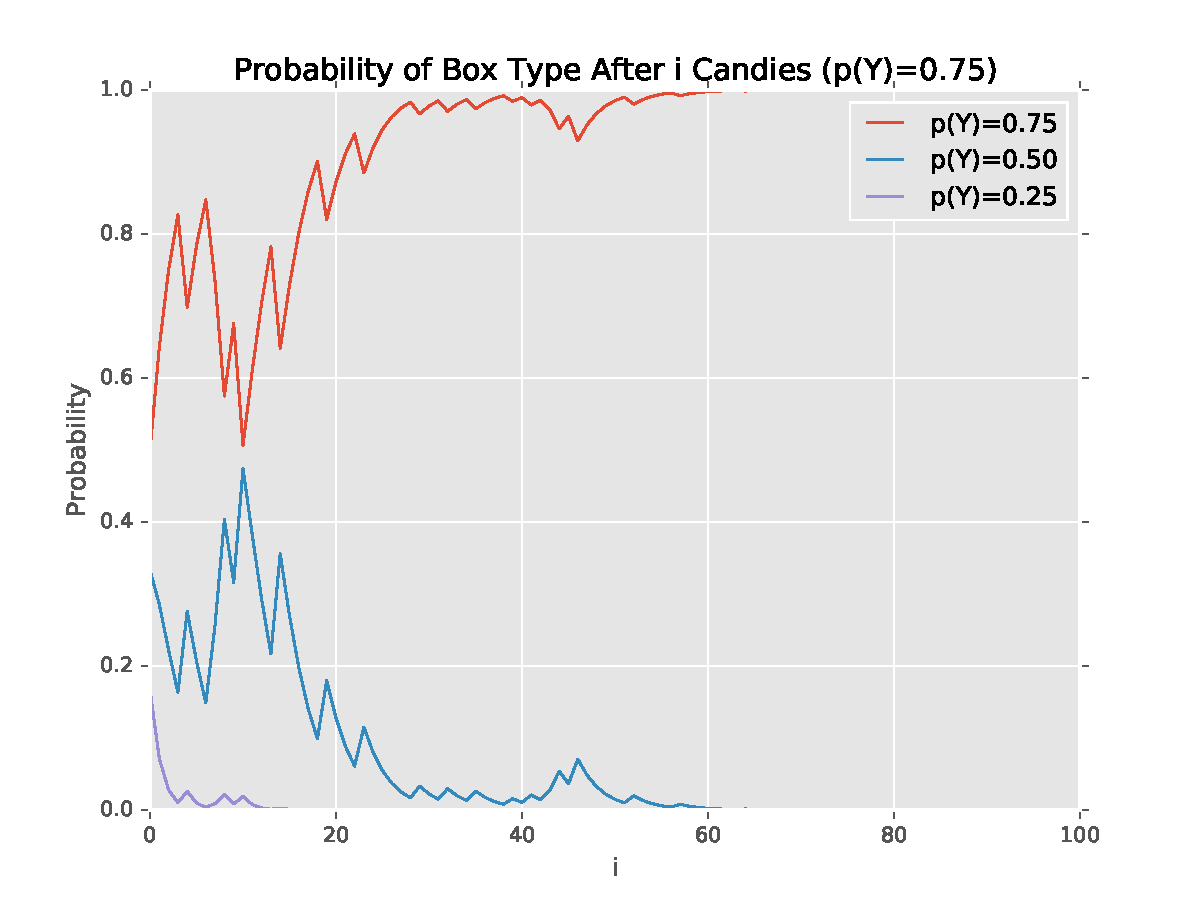
\includegraphics[width=0.5\textwidth]{p1_part1_0_75.pdf}
      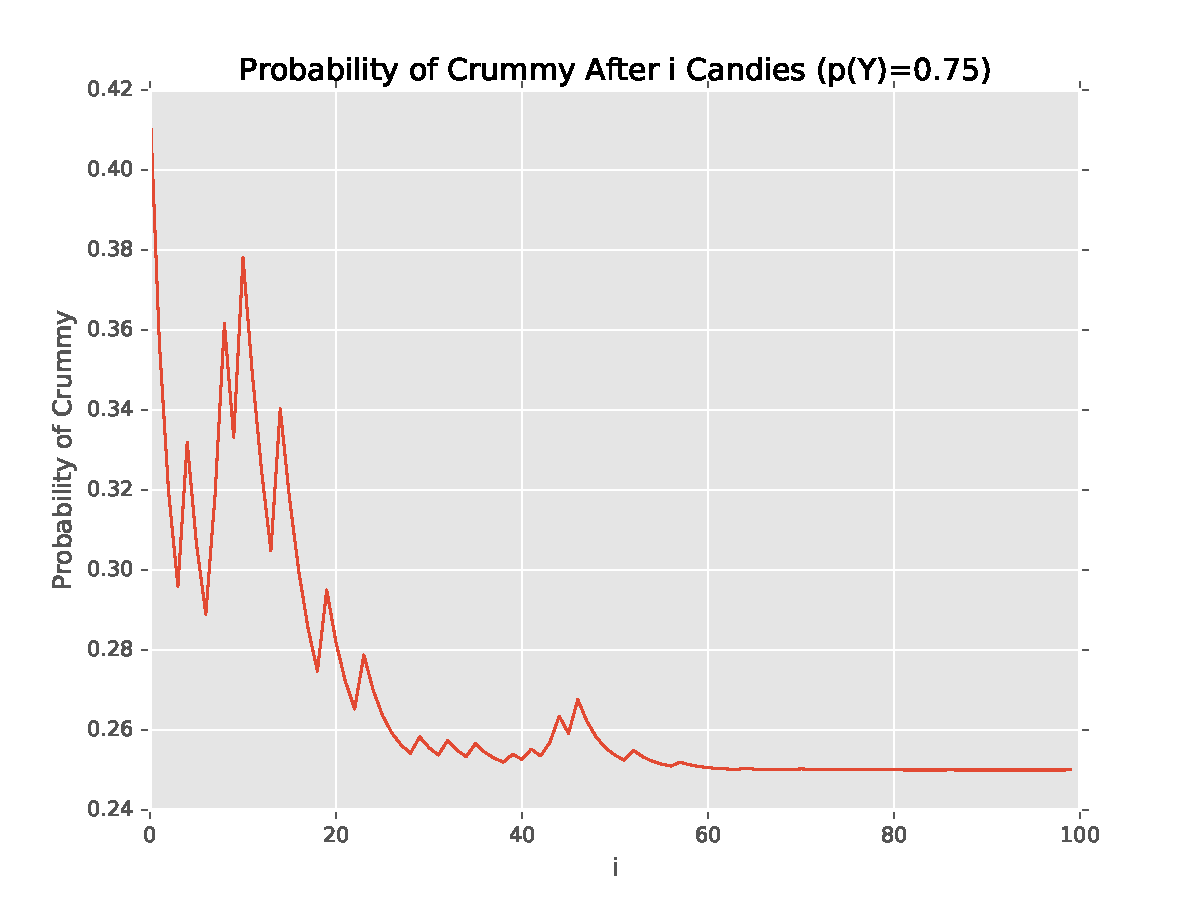
\includegraphics[width=0.5\textwidth]{p1_part2_0_75.pdf}

      For the box type 2 ($p(Y)=0.50$):

      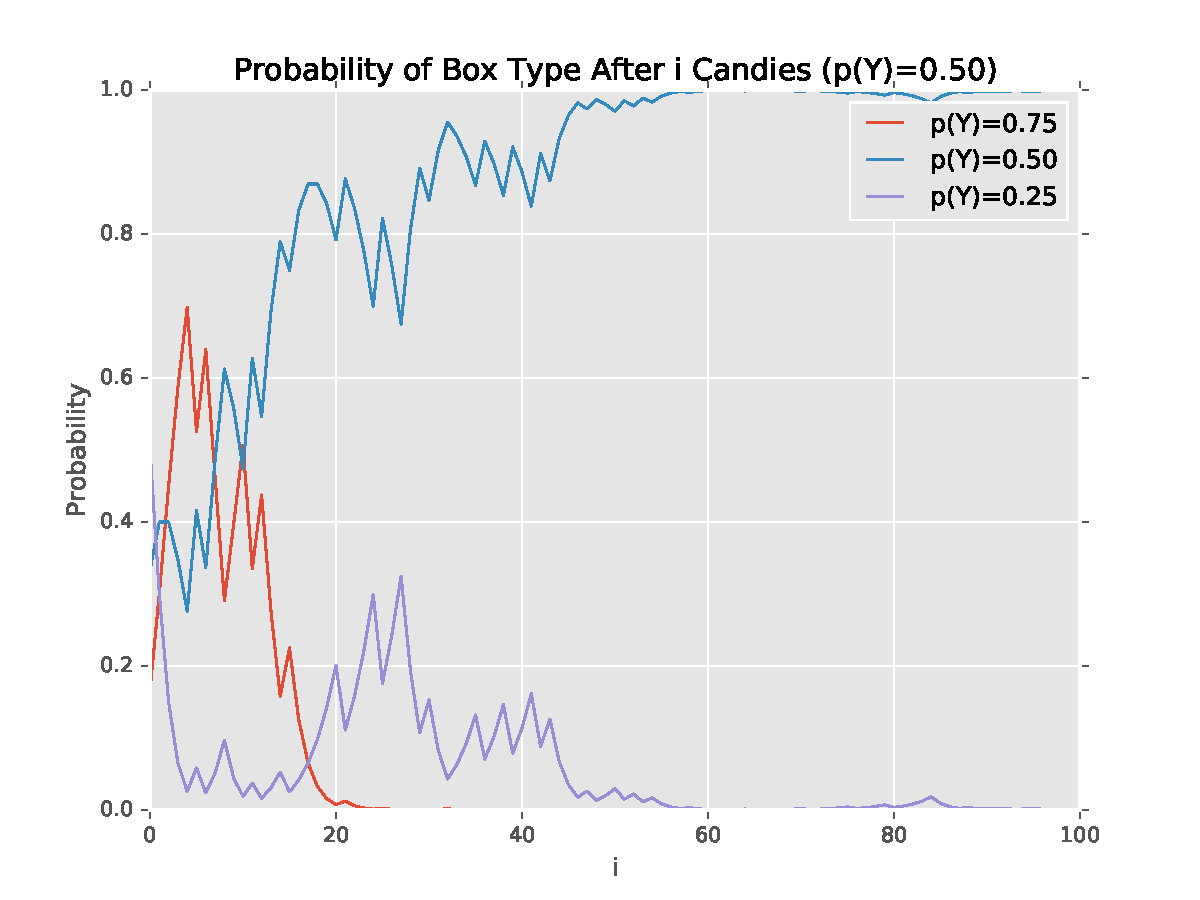
\includegraphics[width=0.5\textwidth]{p1_part1_0_50.pdf}
      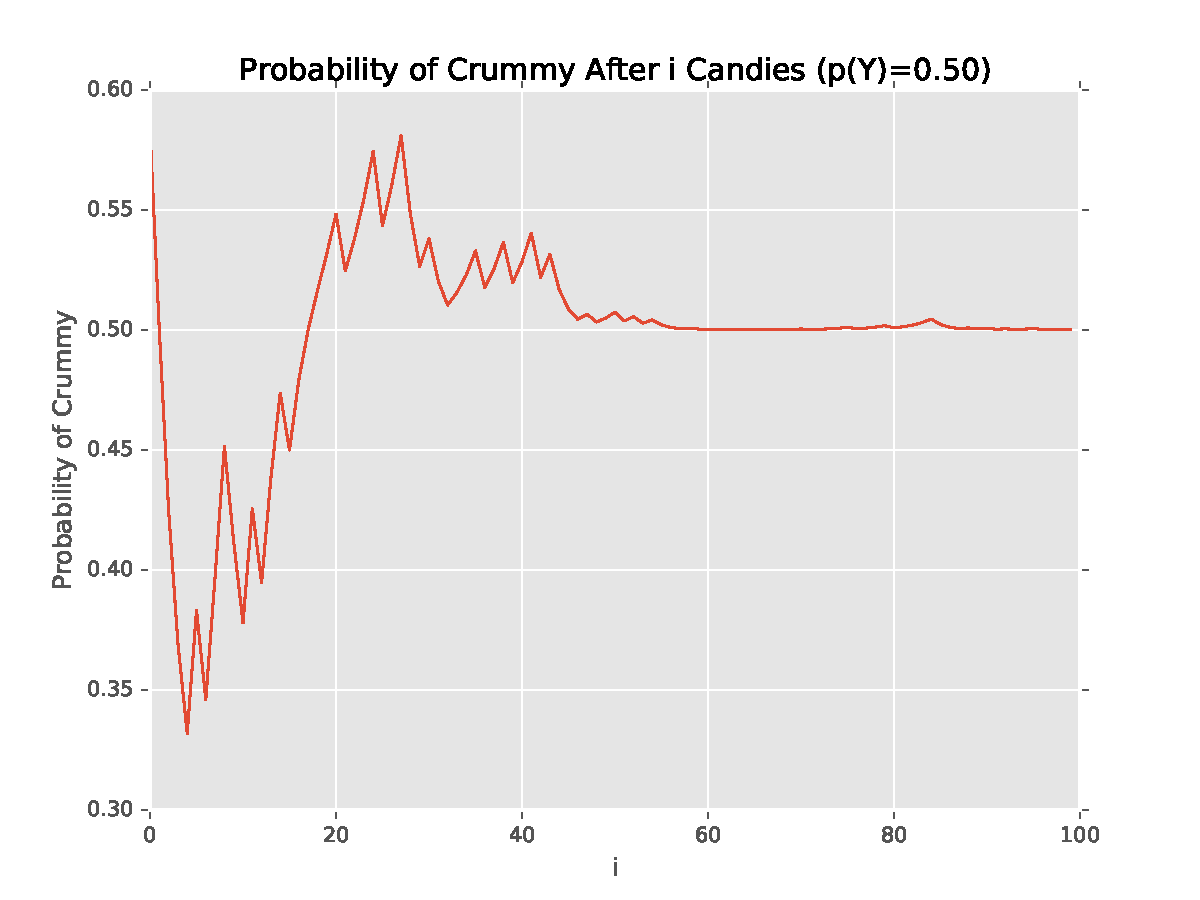
\includegraphics[width=0.5\textwidth]{p1_part2_0_50.pdf}

      For the box type 3 ($p(Y)=0.25$):

      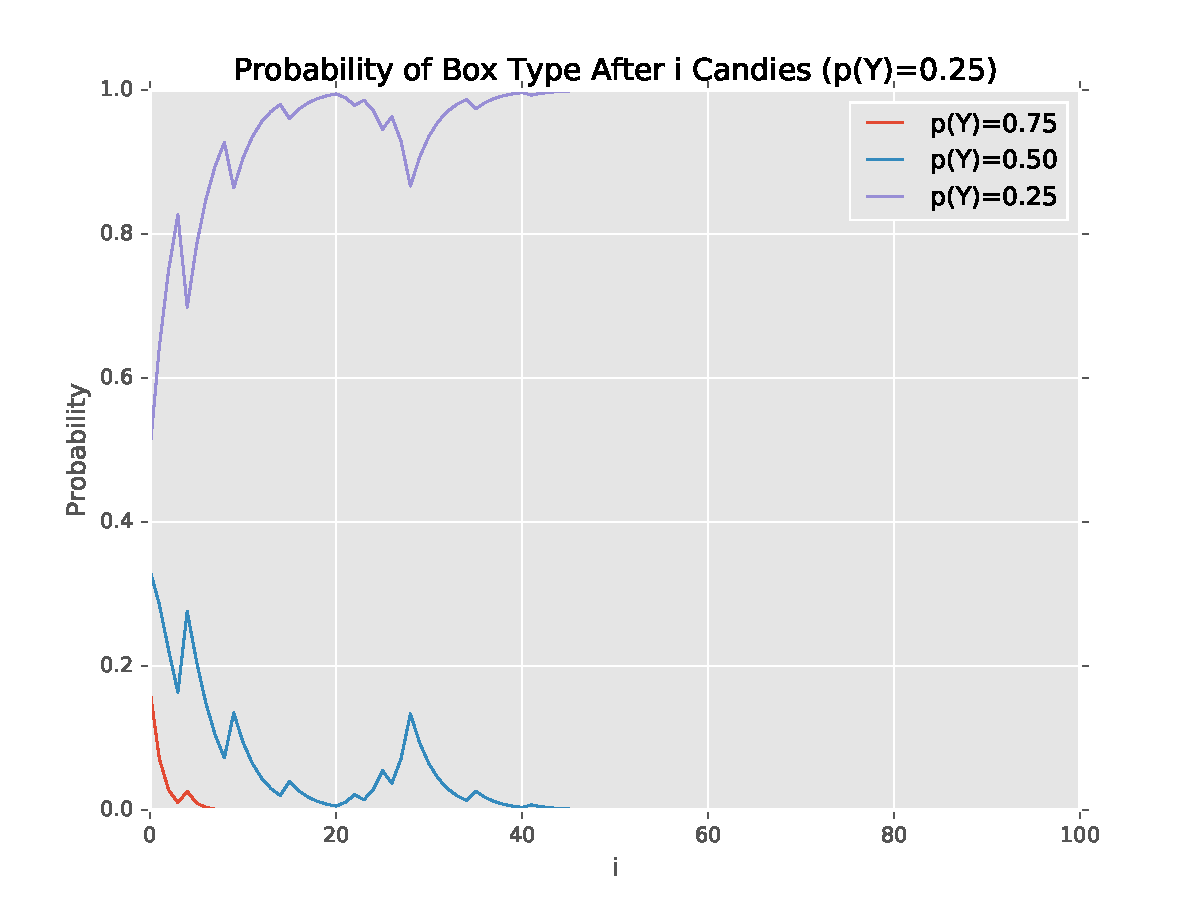
\includegraphics[width=0.5\textwidth]{p1_part1_0_25.pdf}
      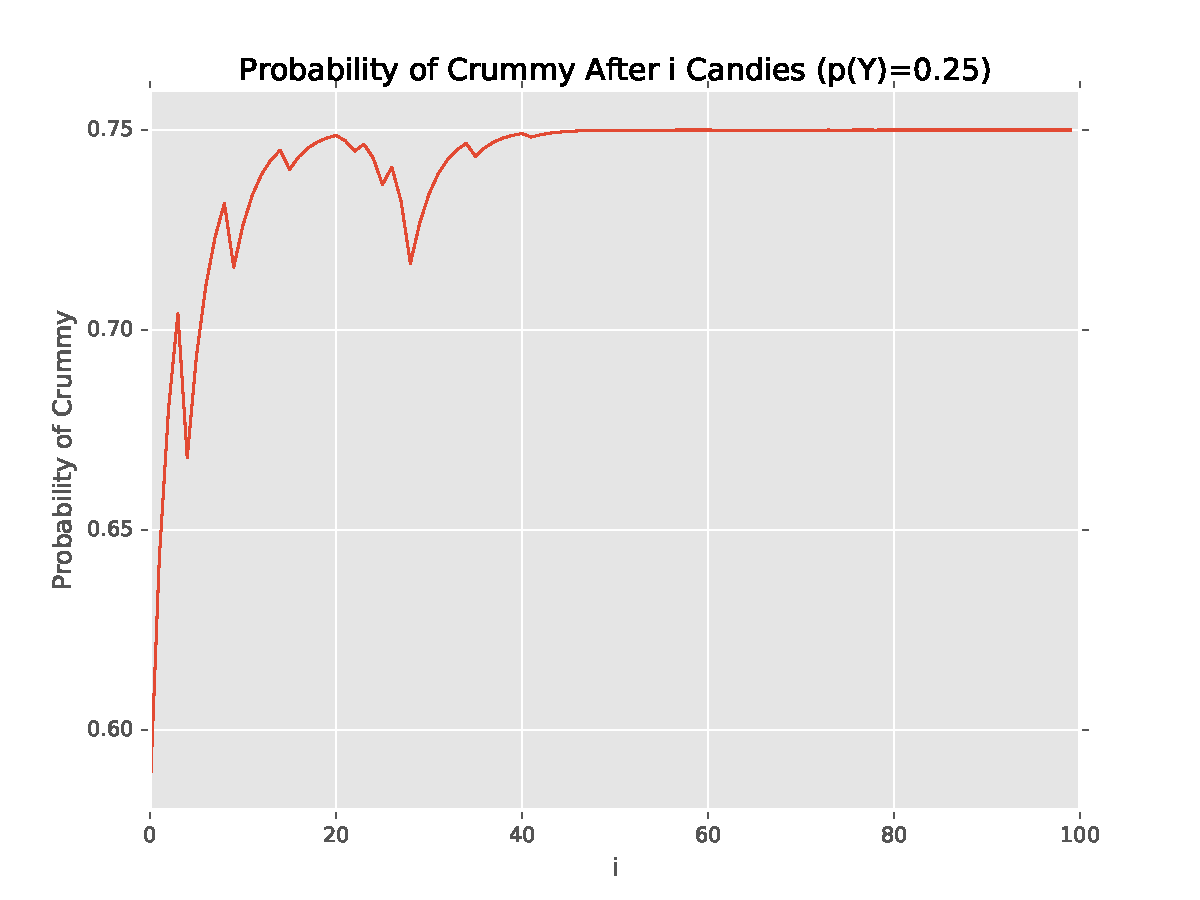
\includegraphics[width=0.5\textwidth]{p1_part2_0_25.pdf}

    \item When we adjust our priors, we obtain the following figures.  For the
      box type 1 ($p(Y)=0.75$):

      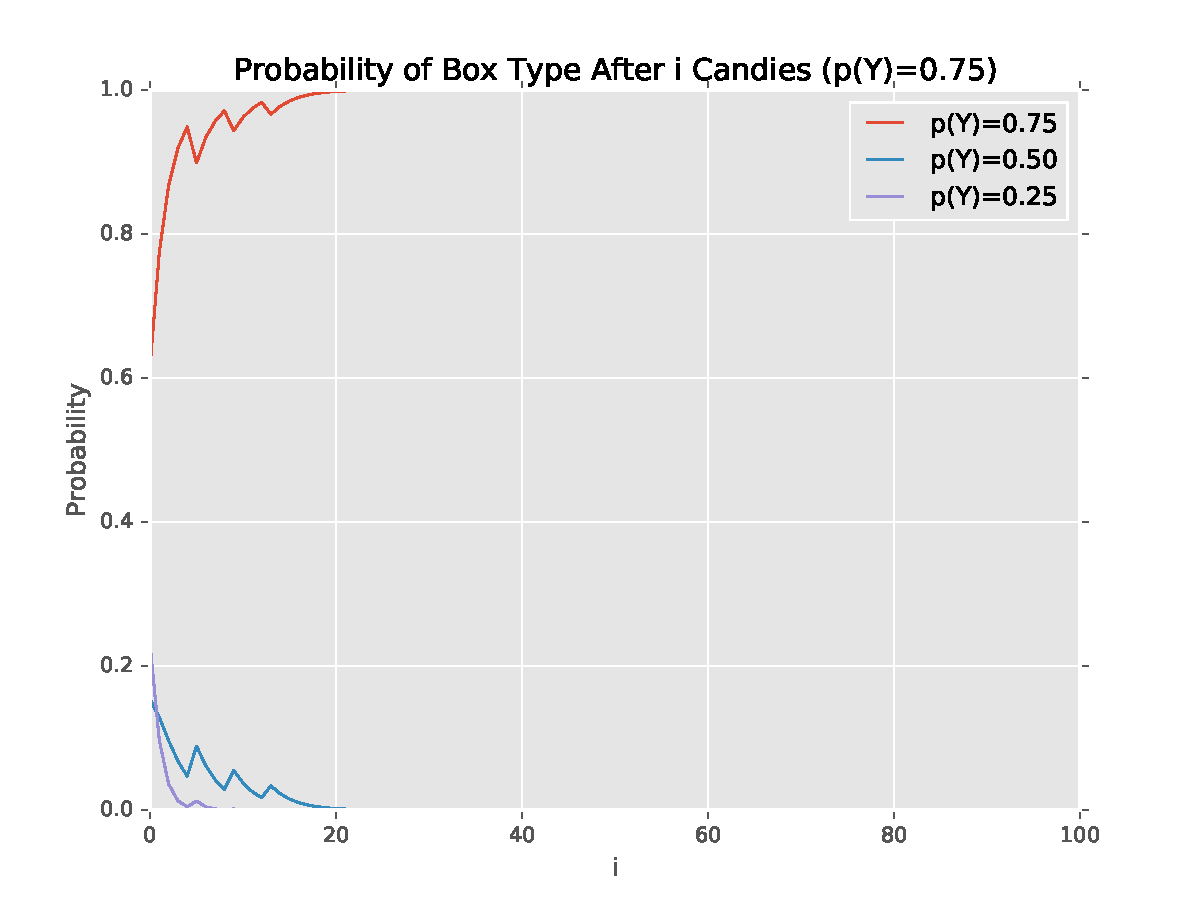
\includegraphics[width=0.65\textwidth]{p1_part3_0_75.pdf}

      For the box type 2 ($p(Y)=0.50$):

      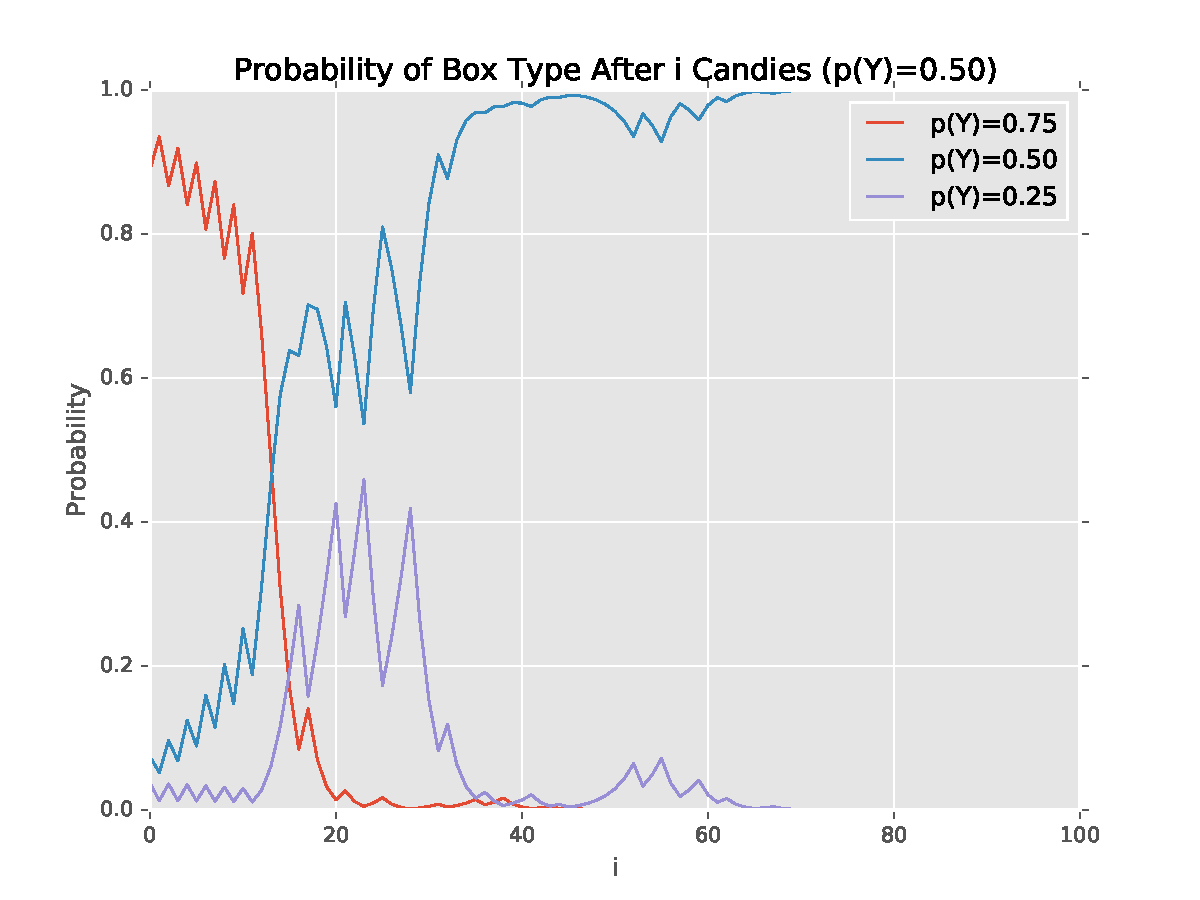
\includegraphics[width=0.65\textwidth]{p1_part3_0_50.pdf}

      For the box type 3 ($p(Y)=0.25$):

      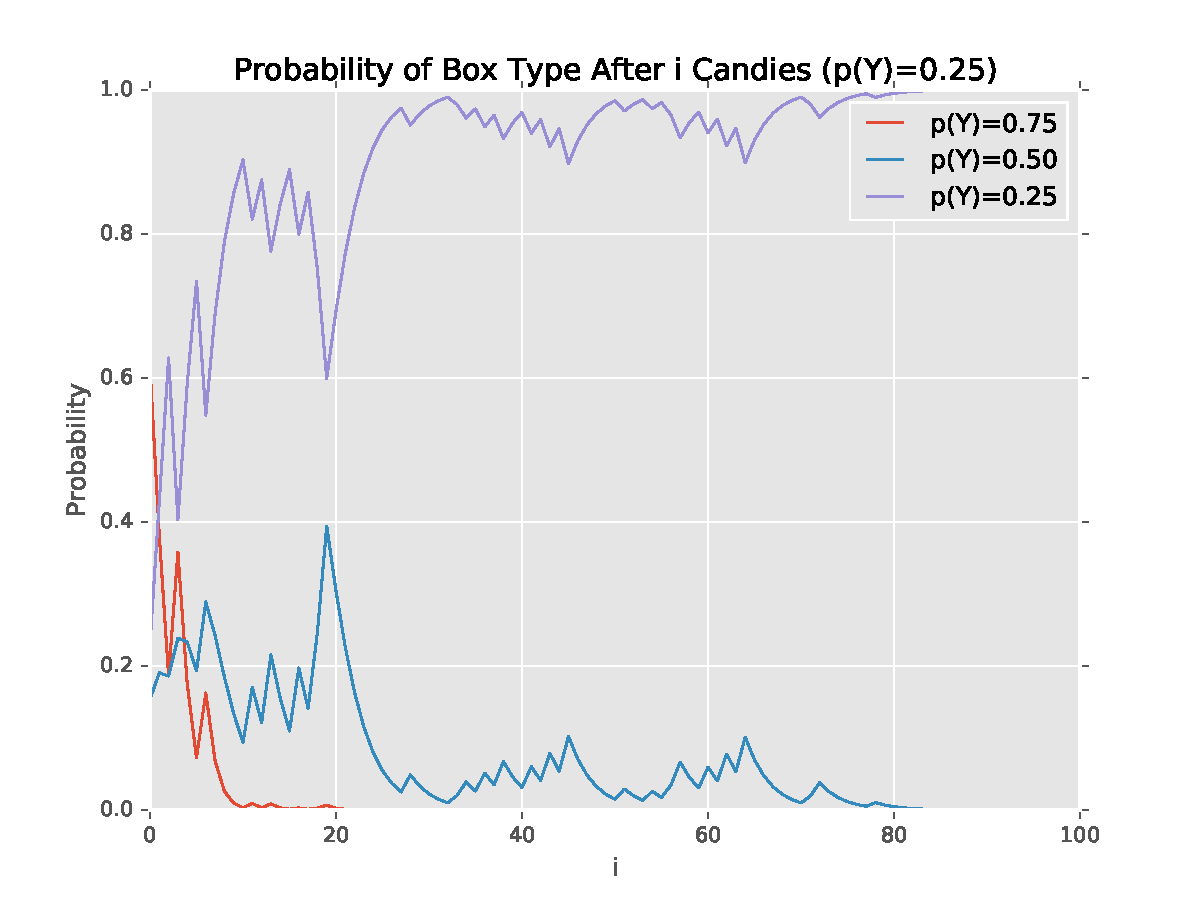
\includegraphics[width=0.65\textwidth]{p1_part3_0_25.pdf}
    \end{enumerate}

    As the figures above demonstrate, the ``optimism'' has a significant effect
    on the number of candies required to ``decide'' which type the box is.  When
    the box is type 1, the probability of box 1 is nearly exactly 1 after only
    20 candies, and it is significantly higher than the other probabilities for
    the entire curve.  Meanwhile, the other types take much longer to
    ``decide'', especially for type 2, since that is easiest to ``confuse'' with
    type 1.
  \end{problem}

  \begin{problem}{2}
    \begin{question}
      When estimating parameters for a Boolean attribute $f$ in a na\"ive Bayes
      model, it is observed that $f$ is true in $k$ out of $n$ positive
      examples. Further, there is a Dirichlet prior on the parameter
      representing the probability of $f$ given a positive example, with
      hyper-parameters $a$ and $b$. Show that the MAP estimate of the
      parameter’s value is equivalent to an $m$-estimate with specific values of
      $m$ and $p$. In this way show that $m$-estimates act as Bayesian prior
      knowledge in na\"ive Bayes. The Dirichlet distribution over
      $0 \le \theta \le 1$ is given by:
      $D(\theta;a,b)=[(a-1)! (b-1)! /(a+b-1)!] \theta^{(a-1)} (1-
      \theta)^{(b-1)}$
      where $a$, $b$ are positive integers greater than 1 and are parameters of
      the distribution. (15 points)
    \end{question}
  \end{problem}

  \begin{problem}{3}
    \begin{question}
      Consider a regression problem with examples described by 2 continuous
      attributes, $x$ and $y$.  Each example is sampled according to the uniform
      distribution on $(-1,1)^2$ and labeled with $f(x,y)=1 - x^2 - y^2$ . A
      learner’s hypothesis class is $h(x,y)=ax+by+c$. (a) Calculate its bias and
      variance as a function of $x$ and $y$ if the learner sees an arbitrarily
      large training sample. (b) Using MATLAB, find the $(x,y)$ with the largest
      bias and the $(x,y)$ with the largest variance for samples of size 10. Can
      you intuitively justify your findings? (15 points)
    \end{question}
  \end{problem}

  \begin{problem}{4}
    \begin{question}
      Suppose a learner uses bootstrap resampling to construct a training sample
      $T$ from an initial sample $U$, of the same size as $U$. Show that, for a
      large enough $U$, the probability that some example from $U$ appears in
      $T$ is approximately 0.63. (5 points)
    \end{question}
  \end{problem}

\end{document}